\documentclass{beamer}
\usepackage[utf8]{inputenc} 
\title{Miasto Hulczyn}
\author{Bartosz Nowaczewski}
\institute{UWM}
\date{\today}
\usepackage{amsfonts}
\usepackage[MeX]{polski}
\begin{document}
\frame{\titlepage}



\begin{frame}
\frametitle{Spis Treści}
\tableofcontents
\end{frame}


\section{1.Ogólne informacje}
\begin{frame}{Ogólne informacje}
\begin{itemize}
\item{Hulczyn to miasto na Śląsku Opawskim, w kraju morawsko-śląskim, na wschodzie Czech, przy granicy z Polską.}
\pause
\item Powierzchnia:  
$${21,13 km^2}$$
\pause
\item Populacja(2012r):
$${14 122}$$
\end{itemize}
\end{frame}

\begin{frame}{Położenie na mapie kraju morawsko-śląskiego}
\begin{figure}
\centering
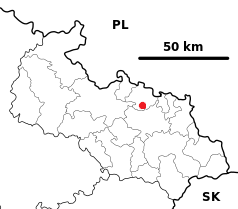
\includegraphics[scale=0.9]{Grafika/Polozenie.png}
\end{figure}
\end{frame}

\section{2.Podział}
\begin{frame}{Podział}
\begin{itemize}
\item{Miasto podzielone jest na trzy części stanowiące również trzy gminy katastralne:}
\pause
\item{Bobrovníky (niem. Bobrownik, Biberswald (od 1939 r.)}
\pause
\item{Darkovičky (niem. Klein Darkowitz)}
\pause
\item{Hulczyn}
\end{itemize}
\end{frame}

\section{3.Historia}
\begin{frame}{Historia}
\begin{itemize}
\item{Założone przez Przemysła Ottokara II w 1256. Należało do księstwa raciborskiego, od 1742 wraz z niemal całym Śląskiem do Prus, od 1816 w powiecie raciborskim prowincji śląskiej Prus.}
\pause
\item{10 stycznia 1920 z mocy traktatu wersalskiego wraz z kraikiem hulczyńskim przyłączone do Czechosłowacji. Po Układzie Monachijskim z 1938 znalazł się w Niemczech do 1945.}
\pause
\item{Odsetek niemieckich mieszkańców w poszczególnych latach: 1890 (18,2\%), 1900 (28,2\%), 1910 (24,2\%), 1921 (30,3\%), 1930 (10,2\%) ^[^ 1^] .}
\end{itemize}
\end{frame}

\section{4.Przypisy}
\begin{frame}{Przypisy}
\begin{thebibliography}{99}
\textit{[1]Barbora PETŘÍKOVÁ: NÁRODNOSTNÍ A NÁBOŽENSKÁ STRUKTURA OBYVATELSTVA HLUČÍNSKA. Olomouc: 2010, s. 34. (cz.)}
\end{thebibliography}
\end{frame}

\section{5.Bibliografia}
\begin{frame}{Bibliografia}
\begin{thebibliography}{99}
\textit{Felix Triest: Topographisches handbuch von Oberschliesen. Breslau: Verlag von Wilh. Gottl. Korn, 1865.}
\end{thebibliography}
\end{frame}
\begin{frame}{Koniec}
\begin{itemize}
\LARGE
{Dziękuję za uwagę}
\end{itemize}
\end{frame}
\end{document}
